\documentclass[11pt]{article}
\usepackage[margin=1in]{geometry}
\usepackage{amsmath,amssymb,graphicx,booktabs,natbib}
\usepackage[colorlinks=true,allcolors=blue]{hyperref}
\setlength{\emergencystretch}{1em}
\hypersetup{pdftitle={When History Can Replace Action Chunking},pdfauthor={Nihar Ballamudi and Kyle Horton}}
\title{When History Can Replace Action Chunking:\\Theory and Recovery Experiments}
\author{Nihar Ballamudi and Kyle Horton\\University of Pennsylvania}
\date{November 5, 2026 --- integrated working draft}
\newcommand{\norm}[1]{\left\lVert#1\right\rVert}
\newcommand{\spr}{\operatorname{spr}}
\begin{document}
\maketitle
\begin{abstract}
We combine exact action recovery from finite observation--action histories, a history-based chunk-stability proposition supplied by Kyle Horton, and the current challenging-pair recovery experiments. Sufficient observability permits exact noiseless one-step imitation but does not identify a controller from restricted demonstrations. We give a conditional contraction certificate for general learners and an explicit small-gain certificate for the rank-one ridge learner. The latter explains why history sixteen permits stable one-step execution in the present noiseless sweep, whereas history eight requires longer commitment under the chosen loss criterion. These conclusions separate information recovery, learning, and feedback stability; they do not assert universal monotonicity of tracking loss.
\end{abstract}
\noindent\textbf{Keywords:} Imitation learning, observability, action chunking, incremental stability.

\section{Question and mathematical setting}
Restricted demonstrations can leave corrective behavior unidentified even when the plant and expert are stable \citep{simchowitz2025}. Action chunking can exploit stable open-loop dynamics to limit error amplification \citep{zhang2025}. We ask when additional history makes frequent replanning reliable, reducing the need for commitment.

Consider $x_{t+1}=Ax_t+Bu_t+w_t$, $y_t=Cx_t$, and expert $u_t^*=Kx_t$; write $F=A+BK$. Schur stability of $A$ concerns decay under common inputs, whereas stability of $F$ concerns expert feedback. The expert is Markovian in $x$; the learner observes
\[
z_t^{(r)}=\operatorname{col}(y_{t-r+1:t},u_{t-r+1:t-1}).
\]
Context $r$ counts observations, prediction horizon $H$ counts predicted actions, and execution length $\ell\le H$ counts committed actions. At $b=j\ell$, the learner predicts a chunk and applies $u_{b+k}=\pi_k(z_b)$ for $0\le k<\ell$. New measurements do not revise that chunk. Reconstruction statements assume $w=0$, known applied inputs, and a valid initial history. The following results are elementary control derivations for this project, not novelty claims about observability.

\section{History and exact imitation}
Let $\mathcal O_r=\operatorname{col}(C,CA,\ldots,CA^{r-1})$ and $h=\min\{r:\operatorname{rank}\mathcal O_r=n\}$ for an observable pair. With $s=t-r+1$, unrolling gives $Y=\mathcal O_rx_s+\mathcal T_rU$ and $x_t=A^{r-1}x_s+\mathcal R_rU$. Here $Y,U$ stack the observed outputs and applied inputs, $\mathcal R_r=[A^{r-2}B\ \cdots\ B]$, and $(\mathcal T_r)_{ij}=CA^{i-1-j}B$ for $j<i$, zero otherwise (zero-based blocks).

\textbf{Lemma 1 (reconstruction).} If $r\ge h$, then $x_t=R_rz_t$, where
\begin{equation}
R_r=[A^{r-1}\mathcal O_r^\dagger\quad\mathcal R_r-A^{r-1}\mathcal O_r^\dagger\mathcal T_r].
\label{eq:reconstruction}
\end{equation}
\emph{Proof.} Recover $x_s=\mathcal O_r^\dagger(Y-\mathcal T_rU)$ and propagate to $t$. $\square$ The input correction is essential; the identity holds under arbitrary learner actions.

\textbf{Proposition 1 (action recovery).} A policy satisfying $\pi_r(z_t)=Kx_t$ for every noiseless history exists if and only if
\begin{equation}\ker\mathcal O_r\subseteq\ker(KA^{r-1}).\label{eq:kernel}\end{equation}
\emph{Proof.} Under identical inputs, indistinguishable histories have initial-state difference $d\in\ker\mathcal O_r$ and current-action difference $KA^{r-1}d$. Necessity follows. Conversely, kernel inclusion makes $\mathcal O_rx_s\mapsto KA^{r-1}x_s$ a well-defined linear map; add the known input contribution. $\square$

Full observability is sufficient but not necessary: only action-relevant information must be recovered. If \eqref{eq:kernel} fails, indistinguishable histories require actions separated by some $\Delta\ne0$. Every deterministic predictor errs by at least $\norm{\Delta}/2$ on one history. The first action of any chunk obeys the same lower bound. Commitment cannot create missing information. In fact, exact prediction of an entire $\ell$-action expert chunk requires
\[
\ker\mathcal O_r\subseteq\bigcap_{k=0}^{\ell-1}\ker(KF^kA^{r-1}),
\]
since its $k$th action is $KF^kx_t$. Longer prediction can demand more information than the current action alone.

\textbf{Proposition 2 (execution equivalence).} For $r\ge h$, the policy $\pi_k^*(z)=KF^kR_rz$ reproduces the noiseless expert trajectory for every $1\le\ell\le H$. Consequently, if $F$ is Schur stable, exact single-step imitation is stable.

\emph{Proof.} Reconstruction gives the boundary state $x_b$. If $x_{b+k}=F^kx_b$, applying $KF^kx_b$ gives $x_{b+k+1}=F^{k+1}x_b$. Induct within each chunk and repeat at the next boundary. $\square$

Thus sufficient context removes a representational need for chunking, but no horizon is strictly preferable in the exact noiseless case. Learning error and disturbances create the tradeoff. Under shared disturbances, single-step learner--expert tracking error satisfies $d_{t+1}=Fd_t+Be_t$, where $e_t=\hat\pi(z_t)-Kx_t$. If $\norm{F^k}\le M_F\beta^k$, $\beta<1$, and deployment error is bounded by $\varepsilon$, then $\limsup_t\norm{d_t}\le M_F\norm{B}\varepsilon/(1-\beta)$. More explicitly, unrolling gives
\[
\norm{d_t}\le M_F\beta^t\norm{d_0}
+M_F\norm{B}\sum_{i=0}^{t-1}\beta^{t-1-i}\norm{e_i}.
\]
Small training loss does not establish the required deployment bound. If only observations are noisy, reconstruction error is $A^{r-1}\mathcal O_r^\dagger V_t$, where $V_t$ stacks measurement errors. Full rank therefore does not ensure good conditioning or robustness.

\paragraph{Representation versus identification.}
Noiseless expert histories have the form $z_t=S_rx_{t-r+1}$, with $S_r$ stacking $CF^j$ for $0\le j<r$ and $KF^j$ for $0\le j<r-1$. Their feature rank is at most $n$. Any $\Delta W$ satisfying $\Delta WS_r=0$ is invisible on demonstrations but may change behavior on disturbed histories. More context can therefore enlarge the policy class without identifying its off-demonstration behavior. Process noise also invalidates exact deterministic reconstruction.

\section{A stability guarantee for action chunks}
Set $w=0$. Assume that all admissible trajectory pairs satisfy
\begin{equation}
\norm{\delta y_{t+k}}\le C_0\rho^k\norm{\delta z_t}_{\mathcal Z}
+C_0\sum_{i=0}^{k-1}\rho^{k-1-i}\norm{\delta u_{t+i}},
\label{eq:ios}
\end{equation}
where $C_0\ge1$, $0<\rho<1$, and $\norm{z}_{\mathcal Z}$ sums block Euclidean norms. For observable Schur-stable plants and $r\ge h$, this follows from Lemma 1 and $\norm{A^k}\le M_A\rho^k$, with $C_0$ enlarged to bound the output and input maps. Observability alone does not imply decay.

\textbf{Proposition 3 (history-based chunk stability).} Use the same policy and schedule on both trajectories, with $u_{j\ell+k}=\pi_k(z_{j\ell})+v_{j\ell+k}$ and $\operatorname{Lip}_{\mathcal Z}(\pi_k)\le D\rho^k$. For $0<\alpha<1$, define
\[
\bar\rho=\rho^{1-\alpha},\quad C_r=2rC_0\rho^{-(r-1)},\quad
\bar C=C_0\left(1+\frac{D}{e\alpha\rho\log(1/\rho)}\right).
\]
If $\ell\ge\max(1,r-1)$ and $C_r(1+D\ell/\rho)\rho^{\alpha\ell}\le1$, then
\begin{equation}
\norm{\delta y_t}\le\bar C\bar\rho^t\norm{\delta z_0}_{\mathcal Z}
+\bar CC_r\sum_{i=0}^{t-1}\bar\rho^{t-1-i}\norm{\delta v_i}.
\label{eq:chunkbound}
\end{equation}
\emph{Proof.} Put $Z_j=\norm{\delta z_{j\ell}}_{\mathcal Z}$ and $V_i=\norm{\delta v_i}$. The policy gives $\norm{\delta u_{j\ell+k}}\le D\rho^kZ_j+V_{j\ell+k}$. Substituting in \eqref{eq:ios} yields, for $0\le k\le\ell$,
\[
\norm{\delta y_{j\ell+k}}\le C_0(1+Dk/\rho)\rho^kZ_j
+C_0\sum_{i=0}^{k-1}\rho^{k-1-i}V_{j\ell+i}.
\]
Since $\ell\ge r-1$, all blocks of the next history lie within the chunk, including its initial observation when equality holds. Summing their bounds gives
\[
Z_{j+1}\le C_r(1+D\ell/\rho)\rho^\ell Z_j
+C_r\sum_{i=0}^{\ell-1}\rho^{\ell-1-i}V_{j\ell+i}.
\]
The first coefficient is at most $\bar\rho^\ell$. Iterate, use $\rho\le\bar\rho$, and apply $k\rho^{\alpha k}\le1/[e\alpha\log(1/\rho)]$ to the within-chunk bound to obtain \eqref{eq:chunkbound}. $\square$

Sufficiently long chunks satisfy the condition when $H$ permits them. However, decreasing chunk sensitivity is an assumption, and the bound becomes more conservative as $r$ grows. It does not by itself prove that context permits shorter execution.

\paragraph{Exact linear test and example.}
Augment the state with observation/action buffers: $s_{t+1}=\mathsf As_t+\mathsf Bu_t+\mathsf Jw_t$, $z_t=\mathsf Ps_t$. A fitted linear chunk policy has boundary map
\begin{equation}
M_{r,\ell}=\mathsf A^\ell+\sum_{k=0}^{\ell-1}\mathsf A^{\ell-1-k}\mathsf B\widehat W_k\mathsf P.
\label{eq:lift}
\end{equation}
Unrolling gives the map. The augmented system is exponentially stable exactly when $\spr(M_{r,\ell})<1$. For $x_+=x/2+u$ and expert $K=0$, the imperfect predictor $\pi_k(x)=3\cdot2^{-k}x/4$ gives $M_\ell=2^{-\ell}(1+3\ell/2)$. At $\ell=1,2,3$, the multipliers are $1.25,1,0.6875$. Three-step commitment stabilizes this predictor family; the exact expert still needs no chunking.

\section{Connecting context to reliable execution}
Propositions 1--2 describe an information mechanism: history can recover action-relevant state. Proposition 3, adapted from Kyle Horton's supplied draft with its proof completed and notation standardized, describes a feedback mechanism: sufficiently long commitment controls sensitivity on a stable plant. These mechanisms are complementary. Crucially, Proposition 3 alone does not connect them: $C_r$ increases with $r$, and its restriction $\ell\ge r-1$ cannot certify the observed $r=16,\ell=1$ setting. A sharper learner-dependent argument is needed.

\paragraph{A conditional result for general learners.}
Use any fixed vector norm and its induced operator norm; choose it so that $\norm{F}\le a<1$, possible when $F$ is Schur stable. At a chunk boundary, let an arbitrary deterministic history learner satisfy, on all admissible deployment histories,
\begin{equation}
\norm{\hat\pi_{r,j}(z_t)-KF^jx_t}\le\gamma_r q^j\norm{x_t},\qquad 0<q<1.
\label{eq:relative}
\end{equation}
This is a uniform relative error assumption, not a consequence of small demonstration loss. It excludes additive error at the origin. Nonlinear learners are permitted; the condition concerns their behavior rather than their parameterization.

\textbf{Proposition 4 (conditional context--execution certificate).} Under \eqref{eq:relative}, define
\begin{equation}
G(r,\ell)=a^\ell+\gamma_r\sum_{j=0}^{\ell-1}\norm{A^{\ell-1-j}B}q^j.
\label{eq:certificate}
\end{equation}
If $G(r,\ell)<1$, deployment is exponentially stable at the origin, with contraction factor at most $G(r,\ell)$ per chunk. If $\gamma_r$ is nonincreasing in $r$, the shortest execution length certified over a fixed tested grid is nonincreasing on its feasible domain. In particular, $\gamma_r\norm{B}<1-a$ certifies $\ell=1$.

\emph{Proof.} Write $e_j=\hat\pi_{r,j}(z_t)-KF^jx_t$. Direct unrolling gives
\[
x_{t+\ell}=F^\ell x_t+\sum_{j=0}^{\ell-1}A^{\ell-1-j}Be_j.
\]
Taking norms yields $\norm{x_{t+\ell}}\le G(r,\ell)\norm{x_t}$. The same bound holds at every boundary by the deployment assumption; the finitely many within-chunk maps have bounded gains. Thus exponential decay extends to all phases. At fixed $\ell$, $G$ is nondecreasing in $\gamma_r$, so certified feasible sets expand as $\gamma_r$ decreases. At $\ell=1$, $G=a+\gamma_r\norm{B}$. $\square$

If $A$ is also Schur stable and the same geometric prediction-error envelope extends to arbitrarily large $H$, then $G(r,\ell)\to0$ as $\ell\to\infty$ at fixed $r$. Indeed $\norm{A^kB}\le M_A\norm{B}\rho_A^k$ and the convolution of the two decaying geometric sequences tends to zero. This is an eventual certificate, not monotonicity of finite test loss or a guarantee within $H=16$.

For bounded additive prediction or reconstruction errors, exact convergence is replaced by practical tracking. At $\ell=1$, if $\norm{\hat x_t-x_t}\le\eta_r$ and $\norm{\hat u_t-K\hat x_t}\le\epsilon_r$, the earlier tracking bound applies with $\varepsilon=\epsilon_r+\norm{K}\eta_r$. Observability makes $\eta_r=0$ representable in the noiseless known-model setting once $r\ge h$; neither observability nor a larger function class guarantees that a trained learner achieves decreasing $\epsilon_r$ or $\gamma_r$. Those require coverage, estimation, conditioning and generalization arguments.

\paragraph{What the general result does not establish.}
The present raw-history ridge learner is not known to satisfy \eqref{eq:relative} uniformly over arbitrary histories. Past states and actions can vary independently of a small current state, so a finite current-state-relative bound need not hold. Proposition 4 is a framework for observer-based or otherwise certified learners, not a theorem already verified by the sweep. Its certificate concerns stability; an execution length selected for low test loss requires a separate performance estimate.

\section{An explicit theory for the narrow-data ridge learner}
For the challenging pair at $\mu=1/8$, let $q=1-2\mu=3/4$ and $c=3\mu/2=3/16$. In this section $q$ is the expert's demonstrated decay rate, distinct from an arbitrary plant-stability rate $\rho$. The construction is from Definition 4.1 of \citet{simchowitz2025}; the following ridge calculation is specific to our experiment.

On every expert demonstration, $x_1=0$, $x_{2,t+1}=qx_{2,t}$, and $u_{1,t}=-cx_{2,t}$, $u_{2,t}=0$. Every feature equals $x_{2,t}v_r$, where $v_r$ contains observation coefficients $q^{-k}$ in the $x_2$ slots ($0\le k<r$), input coefficients $-cq^{-k}$ in the past-$u_1$ slots ($1\le k<r$), and zeros elsewhere. Set
\[
D_r=\norm{v_r}_2^2=1+(1+c^2)\sum_{k=1}^{r-1}q^{-2k},\qquad
S=\sum_i x_{2,t_i}^2>0,\qquad \delta=\lambda/S.
\]
For $b_H=\operatorname{col}((-cq^j,0))_{j=0}^{H-1}$, the fitted chunk matrix is exactly
\begin{equation}
\widehat W=\frac{b_Hv_r^\top}{D_r+\delta}.
\label{eq:ridgeexact}
\end{equation}
\emph{Derivation.} The regression matrices are $X=s v_r^\top$, $Y=s b_H^\top$. Solving $(X^\top X+\lambda I)\widehat W^\top=X^\top Y$ gives \eqref{eq:ridgeexact}; the zero-penalty formula is the minimum-norm limit. This also explains why prediction horizons overlap at a fixed executed prefix when input windows are matched.

For one-step execution, the learned policy is therefore
\begin{equation}
 u_{1,t}=-\frac{c}{D_r+\delta}\sum_{k=0}^{r-1}q^{-k}x_{2,t-k}
 +\frac{c^2}{D_r+\delta}\sum_{k=1}^{r-1}q^{-k}u_{1,t-k},\qquad u_{2,t}=0.
\label{eq:ridgepolicy}
\end{equation}
History does not increase feature rank or identify $K\mathbf e_1$. It changes the minimum-norm extension off the demonstrated histories.

\textbf{Proposition 5 (sufficient history for ridge stability without chunking).} Define
\[
\alpha_r=\frac{c\sum_{k=0}^{r-1}q^{-k}}{D_r+\delta},\qquad
\beta_r=\frac{c^2\sum_{k=1}^{r-1}q^{-k}}{D_r+\delta}.
\]
The one-step ridge controller is asymptotically stable on plant $A_1$ whenever
\begin{equation}48\alpha_r+\beta_r<1.\label{eq:smallgain}\end{equation}
In particular, sufficiently long history stabilizes the zero-penalty minimum-norm controller, and the same sufficient condition is conservative for positive ridge penalty.

\emph{Proof.} Write $A_1=aI+N$, $a=15/16$, with $N^2=0$ and $N_{21}=-c$. The plant's scalar transfer from $u_1$ to $x_2$ has absolute impulse-response sum
\[
\sum_{k\ge0}|\mathbf e_2^\top A_1^k\mathbf e_1|
=c\sum_{k\ge1}k a^{k-1}=\frac{c}{(1-a)^2}=48.
\]
The observation and autoregressive filters in \eqref{eq:ridgepolicy} have coefficient sums $\alpha_r$ and $\beta_r$. The combined strictly causal feedback map thus has absolute convolution gain at most $48\alpha_r+\beta_r$. If this is below one, its inverse has a convergent Neumann series; the finite-dimensional closed loop is stable. All remaining plant and buffer modes are stable. Finally $D_r=\Theta(q^{-2r})$, whereas both numerators are $O(q^{-r})$, so $\alpha_r,\beta_r=O(q^r)$. $\square$

At $\delta=0$, the left side of \eqref{eq:smallgain} is $4.9066$, $1.8536$ and $0.2021$ at $r=4,8,16$, respectively. Thus $r=16$ has an analytic one-step stability certificate. A failed sufficient test at $r=8$ is not an impossibility result. This theorem explains an eventual history benefit on this particular stable plant; it does not prove monotone loss improvement, identify the expert, or apply to arbitrary unstable plants. State and action scaling also affect ridge's implicit selection.

At fixed $r$, \eqref{eq:ridgeexact} gives $\hat u_{t+j\mid t}=q^j\hat u_{t\mid t}$. If extended beyond the tested prediction horizon, the exact boundary map tends to zero as $\ell\to\infty$: the plant's free response and its response to the geometrically decaying committed sequence both vanish, and all final buffer entries vanish. Hence sufficiently long commitment also stabilizes this idealized predictor. This explains two possible routes to stability without asserting an ordering of every finite $\ell$.

\section{Retained midterm evidence: partial observation}
The following results are retained from the existing midterm report and were not rerun for this synthesis. Those simulations use stable $A=0.995P_n$, $B=b$, $K=-0.05b^\top P_n$, where $P_n$ is a cyclic permutation and $b$ a unit vector. Ridge fits use 32 noiseless demonstrations, 24 matched windows each, penalty $10^{-6}$, and $H=16$. Three seeds each supply eight paired episodes with shared initial states and process noise of coordinate standard deviation $0.02$. After a common $n$-step expert warm-up, tail error averages $\norm{x_t-x_t^*}^2/n$ over the last 200 of 600 steps. Output-separable regression makes the first-action fit identical across prediction horizons, isolating the effect of execution.

\begin{center}\small
\begin{tabular}{ccrr}\toprule
Context $r$ & Execution $\ell$ & Mean tail MSE & Max. per-step rate\\\midrule
3&1&$\infty$&1.3215\\
3&2&$2.80\times10^{-4}$&0.9923\\
4&1&$7.64\times10^{-6}$&0.9923\\
4&16&$5.55\times10^{-5}$&0.9923\\\bottomrule
\end{tabular}
\end{center}
For $n=10,h=4$, the table reports rates $\spr(M_{r,\ell})^{1/\ell}$. At $r=3$, validation MSE is $4.62\times10^{-14}$ despite failure in all 24 single-step rollouts. Two-step commitment stabilizes the fit; context four enables single-step execution with $37\times$ lower tracking error. Across 20 dimension/sensor configurations, single-step execution is best in mean tail error in 19 cases at $r=h$. These observations illustrate the mechanisms, not Proposition 3's policy-class assumptions.

\section{Current pitfalls results: a separate recovery experiment}
The focused sweep in \texttt{pitfalls/chunk\_sweep.py} fixes plant $A_1$ and full observations $C=I$, so its observability index is $h=1$. It varies $r\in\{1,2,4,8,16\}$ and $H,\ell\in\{1,2,4,8,16\}$ with $\ell\le H$. Each of five training seeds supplies 32 narrow noiseless demonstrations. Both target times and sample counts are matched across $r$ and $H$, with ridge penalty $10^{-6}$. There are 375 learned configurations.

A separate RNG generates 20 held-out pairs of initial states. Each pair shares $x_2\sim\mathrm{Unif}[-1,1]$; one state has $x_1=0$, the other a random-sign perturbation of magnitude uniform on $[0.0005,0.0015]$. All controllers use the same 40 states. A common 15-step on-support expert history is supplied and the departure is injected at deployment, so warm-up cannot remove it. There is no continuing noise. The main loss averages squared full-state tracking distance from the expert over 200 post-action states, then over the 20 perturbed rollouts. Support loss is saved separately. A 1000-step canonical rollout from $[0.001,1]$ is a diagnostic, not another test-set mean.

\begin{center}\small
\begin{tabular}{rrrrr}\toprule
$r$ & $\ell$ & Median test MSE & Worst per-step rate & Shortest passing $\ell$\\\midrule
1&1&$9.108\times10^{12}$&1.12498&None\\
2&1&$6.178\times10^{9}$&1.10405&None\\
4&16&$1.379\times10^{-5}$&1.00548&None\\
8&1&$7.396\times10^{-4}$&1.01892&8\\
8&8&$2.260\times10^{-6}$&0.99544&8\\
16&1&$6.487\times10^{-7}$&0.97110&1\\\bottomrule
\end{tabular}
\end{center}
All rows use $H=16$. Passing requires every training seed to have mean test MSE on perturbed states at most $10^{-5}$ and exact boundary spectral radius below one. This illustrative absolute tolerance is not a paper-prescribed threshold; it is sensitive to perturbation scale and rollout length. None means no tested execution passes, not impossibility. Medians summarize the five training seeds; these are not confidence guarantees.

\begin{figure}[htbp]
\centering
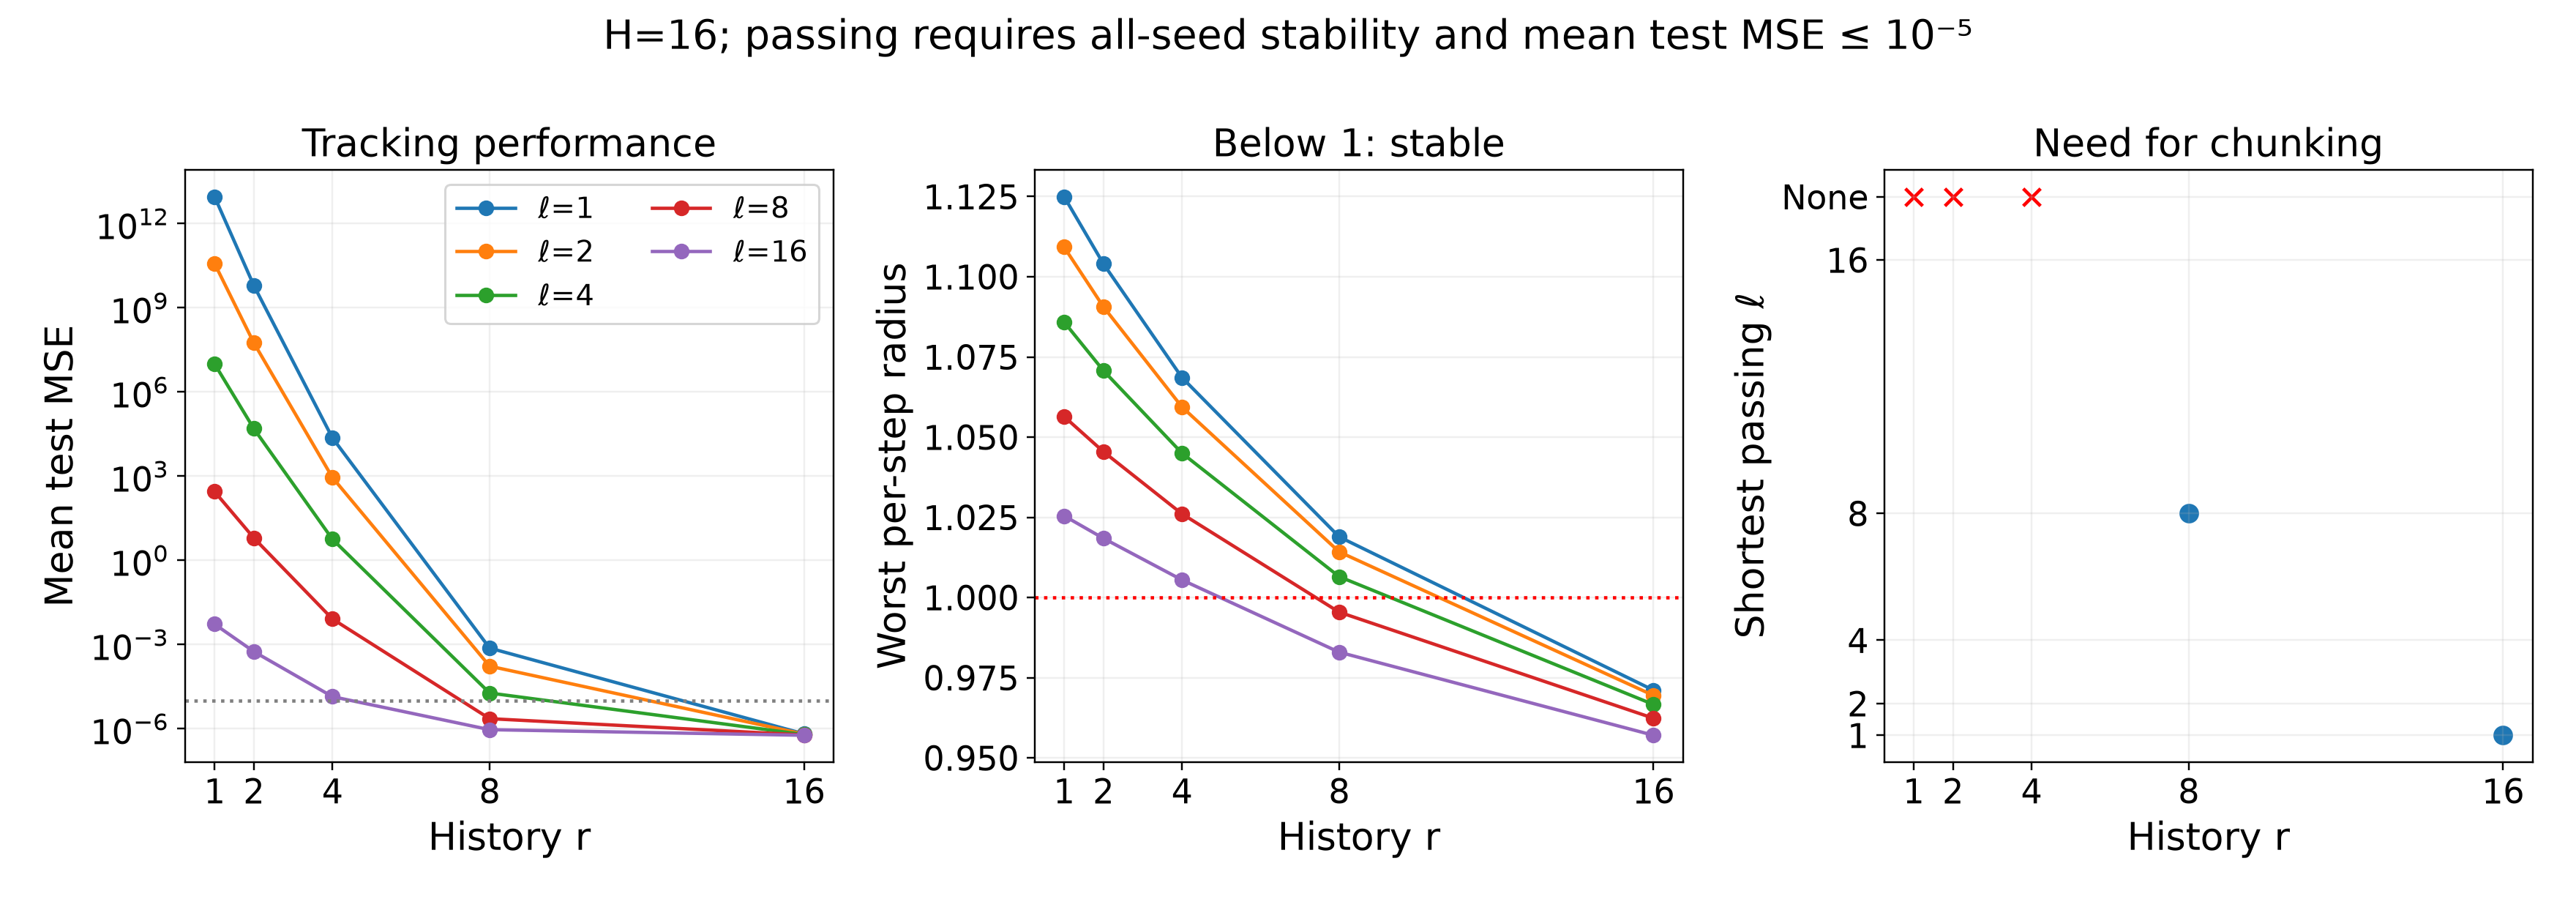
\includegraphics[width=\linewidth]{figures/context_hypothesis.png}
\caption{Current recovery sweep: history improves test tracking and exact spectral stability; the shortest passing execution falls from 8 at $r=8$ to 1 at $r=16$. The loss panel shows seed medians and the stability panel worst-seed rates. The criterion concerns means over test states.}
\label{fig:current}
\end{figure}

Static reference mean test losses are zero for $K_1$, $0.08217$ for zero control, and $1.736\times10^{-8}$ for the model-informed analytic memory witness. The $r=16,\ell=1$ learned controller therefore improves tracking substantially over zero control, while remaining worse than the witness. Its improvement is not evidence of resolving hidden state: $h=1$ already. Proposition 5 instead explains stabilization through the history-dependent ridge extension. Prediction-length curves overlap, as expected from output-separable regression.

\paragraph{Reconciling the earlier negative result.}
The existing midterm report's statement that no narrow-data setting passed its criterion described an earlier noisy 200-step sweep with $r\le8$ and RMS tolerance $0.05$. The current result uses no continuing noise, includes $r=16$, matches target times across histories, and uses MSE tolerance $10^{-5}$. These are different protocols. The new result neither reproduces nor refutes the earlier noisy result; both should be labeled with their scope.

\section{Unified conclusion and remaining theorem}
The report supports three distinct claims. First, observation/action history can remove action-relevant ambiguity; sufficient observability permits exact noiseless one-step imitation. Second, chunking can suppress destabilizing sensitivity of an imperfect predictor, as captured by Horton's incremental output-stability proposition. Third, the current narrow ridge example admits a separate small-gain argument showing that sufficiently long history stabilizes one-step execution, and the empirical test loss is also small on the specified held-out set.

The stronger general statement remains conditional: history must decrease a deployment prediction error or sensitivity quantity such as $\gamma_r$, not just training MSE. Proving this for a general learner requires a learning-theoretic coverage and estimation argument. A clean next experiment should vary $h$ while fixing $A,B,K$, compare learned state estimators with exact reconstruction, and measure deployment action errors alongside stability. Noise studies must include observability conditioning and disturbance-feedback delay. Fresh training and test seeds should evaluate the chosen criteria before making population claims. None of the supplied results establishes universal monotonicity of loss in either context or execution length.

\begin{thebibliography}{2}
\bibitem[Simchowitz et al.(2025)]{simchowitz2025}
M. Simchowitz, D. Pfrommer, and A. Jadbabaie.
The pitfalls of imitation learning when actions are continuous.
\emph{arXiv:2503.09722}, 2025.
\bibitem[Zhang et al.(2025)]{zhang2025}
T. T. Zhang, D. Pfrommer, C. Pan, N. Matni, and M. Simchowitz.
Action chunking and exploratory data collection yield exponential improvements in behavior cloning for continuous control.
\emph{arXiv:2507.09061}, 2025.
\end{thebibliography}
\end{document}
